\documentclass[10pt]{article}
\usepackage{graphicx}
\usepackage{amssymb}
\usepackage[fleqn]{amsmath}
\usepackage{nccmath}
\usepackage{cases}
\usepackage{hyperref}
\usepackage{multicol}
\usepackage{pgfplots}
\usepackage{enumitem}
\pgfplotsset{compat=1.18}
\usepackage{float}

\title{\bf Math 114L\@: Problem Set 3}
\author{\bf Owen Jones}
\begin{document}
\maketitle
\section*{Question 1}
induction on terms\\
Base case: $s_1(x)=s_2(x)$ and $s_1(c)=s_2(c)$ because $s_1$ is the same assignment to variable $x$ and constant $c$.\\
Induction hypothesis: Let $\tau_1,\ldots,\tau_n$ be terms where $(s_1,\tau_i)=(s_2,\tau_i)$.\\
Induction step: Let $f$ be a function. $(s_1,f(\tau_1,\tau_2,\ldots,\tau_n))=(f((s_1,\tau_1),(s_1,\tau_2),\ldots,(s_1,\tau_n)))$. 
BY IH $(f((s_1,\tau_1),(s_1,\tau_2),\ldots,(s_1,\tau_n)))=(f((s_2,\tau_1),(s_2,\tau_2),\ldots,(s_2,\tau_n)))=(s_1,f(\tau_1,\tau_2,\ldots,\tau_n))$.\\
Induction on formulas\\
Assume for formulas $\phi$ and $\psi$ $\phi(s_1)=\phi(s_2)$ and $\psi(s_1)=\psi(s_2)$.\\
$M\models \lnot\phi(s_1)$ iff $M\not\models\phi(s_1)\Rightarrow M\not\models\phi(s_2)$ iff $M\models \lnot\phi(s_2)$ by IH.\\
$M\models \phi(s_1)\rightarrow\psi(s_1)$ if $M\models\psi(s_1)$ or $M\not\models\phi(s_1)$ thus $M\models\psi(s_1)\rightarrow M\models\psi(s_2)$ or $M\not\models\phi(s_1)rightarrow M\not\models\phi(s_2)$ thus $M\models\psi(s_2)$ or $M\not\models\phi(s_2)$ so $M\models \phi(s_2)\rightarrow\psi(s_2)$.
$M\models\forall x\phi(x,s_1)$ iff $\phi(x,s_1)$ is true for every assignment $x$. $\phi(x,s_1)=\phi(x,s_2)$ iff $M\models\forall x\phi(x,s_2)$.
\section*{Question 2}
\begin{itemize}
    \item [(1)] $\varphi\equiv\lnot(\forall y\exists x(x+x=y))$
    \item [(2)] $\varphi\equiv(\forall y\exists x(x+y=0))$
    \item [(3)] $\varphi\equiv(\forall y\exists x(x+x=y))$
    \item [(4)] $\varphi\equiv(\forall y\exists x(x+x=y))$
    \item [(5)] let $\psi(z)\equiv (\exists x(x+x=z))$ (z is even).\\ 
    $\varphi\equiv(\exists x_1,x_2\forall y(\psi(x_1+y)\lor\psi(x_2+y)))$
\end{itemize}
\section*{Question 3}
\begin{itemize}
    \item [(1)] $\varphi\equiv(\exists y (\lnot(y\le x)\rightarrow (\forall z(z\le x)\lor(y\le z))))$
    \item [(2)] $\varphi\equiv(\exists y(\lnot(x\le y)))$
    \item [(3)] $\varphi\equiv(\exists y(\lnot(x\le y)))$
\end{itemize}
\section*{Question 4}
\begin{itemize}
    \item [(1)] $(\forall x\lnot E(x,x))\land(\forall y\forall z E(y,z)\rightarrow E(z,y))$
    \item [(2)] $M_1=(G,E)$ where $G$ is given by the graph shown below,\\ 
    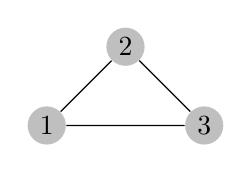
\begin{tikzpicture}
        \tikzstyle{vertex}=[circle,fill=black!25,minimum size=12pt,inner sep=2pt]
  \node[vertex] (G_1) at (-1,-1) {1};
  \node[vertex] (G_2) at (0,0)   {2};
  \node[vertex] (G_3) at (1,-1)  {3};
  \draw (G_1) -- (G_2) -- (G_3) -- (G_1) -- cycle;
    \end{tikzpicture}\\
    $M_2=(G,E)$ where $G$ is given by the graph shown below,\\
    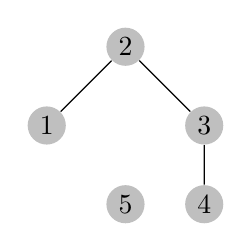
\begin{tikzpicture}
        \tikzstyle{vertex}=[circle,fill=black!25,minimum size=12pt,inner sep=2pt]
  \node[vertex] (G_1) at (-1,-1) {1};
  \node[vertex] (G_2) at (0,0)   {2};
  \node[vertex] (G_3) at (1,-1)  {3};
  \node[vertex] (G_4) at (1,-2)  {4};
  \node[vertex] (G_5) at (0,-2)  {5};
  \draw (G_1) -- (G_2) -- (G_3) -- (G_4) -- cycle;
    \end{tikzpicture}\\
    $M_3=(G,E)$ where $G$ is an undirected tree.
    
\end{itemize}
\section*{Question 5}
\begin{itemize}
    \item [(a)] $\{n:\forall x\forall y((n=x\times y)\rightarrow((x=1)\lor(y=1)))\}$
    \item [(b)] $\{(n,m):\exists x(n=m\times x)\}$
    \item [(c)] $\varphi(m,k)\equiv\exists x(m=k\times x)$\\ 
    $\psi(n)\equiv \forall x\forall y((n=x\times y)\rightarrow((x=1)\lor(y=1)))$\\
    $\{n:\exists x,\exists y,\exists z(\lnot((x=y)\lor(y=z)\lor(x=z))\land(\varphi(n,x\times y\times z))\rightarrow (\psi(x)\land\psi(y)\land\psi(z)))\}$
\end{itemize}
\section*{Question 6}
\begin{itemize}
    \item [(a)] Consider the automorphism $G(x)=-x$. If $\mathbb{N}\subset \mathbb{Z}$ is definable, then $a\in \mathbb{N}$ iff $G(a)\in\mathbb{N}$. 
    This is clearly impossible because the negative numbers are not natural numbers.
    \item [(b)] Consider the automorphism $G(x)=x/2$. If $\mathbb{N}\subset \mathbb{Q}$ is definable, then $a\in \mathbb{N}$ iff $G(a)\in\mathbb{N}$. 
    This is clearly impossible because fractions are not natural numbers.
\end{itemize}
\section*{Question 7}
\begin{itemize}
    \item [(a)] Let $A=\mathbb{N}$ and let $f^M(x)=x$. $\{a\}=\{\exists x(f^M(x)=a)\}$ with $\overline{a}_0=\{a\}$.
    \item [(b)] Let $B=\{-1,1\}$ and let $f^N(x)=x$. 
    $g(x)=-x$ is an automorphism, so $b\in\{b\}$ iff $g(b)\in\{b\}$ which makes $\{1\},\{-1\}$ not definable. 
\end{itemize}
\section*{Question 8}
\begin{itemize}
    \item [(a)] Suppose $|A|\neq|B|$. Because $|A|$ is finite, WLOG let $|A|=n$.
    Consider two L-sentences. 
    $\phi_n:=\forall y(y=x_1\lor y=x_2\lor\ldots \lor y=x_n)$ and $\psi_n:=\exists x_1,\exists x_2,\ldots,\exists x_n(\lnot(x_1=x_2\lor x_1=x_3\lor\ldots\lor x_1=x_n\lor x_2=x_3\lor\ldots\lor x_2=x_n\ldots \lor x_{n-1}=x_n)\land \phi_n)$. 
    If $|B|>|A|$, then $\forall x_1,\forall x_2,\ldots\forall x_n\exists y\lnot(y=x_1\lor y=x_2\lor\ldots \lor y=x_n)$ and if $|B|<|A|$ by the pigeonhole principle $\forall x_1,\forall x_2,\ldots\forall x_n(x_1=x_2\lor x_1=x_3\lor\ldots\lor x_1=x_n\lor x_2=x_3\lor\ldots\lor x_2=x_n\ldots \lor x_{n-1}=x_n)$. Hence, we have found a $\psi_n$ s.t $M\models\psi_n$ and $N\not\models\psi_n$.
    \item [(b)] \begin{itemize}
        \item [(i)] Suppose $V$ and $W$ are isomorphic to each other. 
        It follows there exists some map $T:V\rightarrow W$. 
        Let $\{v_1,v_2,\ldots,v_n\}$ be a basis for $V$. 
        For any $w\in W$, there exists $v\in V$ s.t $w=Tv$.
        $v=\alpha_1v_1+\ldots\alpha_n v_n\Rightarrow w=Tv=T(\alpha_1v_1+\ldots\alpha_n v_n)=\alpha_1Tv_1+\ldots+\alpha_n Tv_n$
        It follows $\{Tv_1,Tv_2,\ldots,Tv_n\}$ forms a basis for $W$.
        Thus, $W$ and $V$ have the same dimension.\\ 
        Suppose $V$ and $W$ have the same dimension.
        Let $\{v_1,v_2,\ldots,v_n\}$ be a basis for $V$ and $\{w_1,w_2,\ldots,w_n\}$ be a basis for $W$.
        We can define an isomorphism $T={[w_1,w_2,\ldots, w_n]}^{-1}[v_1,v_2,\ldots, v_n]$ which is a bijection from $V\rightarrow W$.
        By basic linear algebra, the transformation is linear and preserves $0$. Thus, $V$ is isomorphic to $W$.
        \item[(ii)] From (i) we know that $V$ is isomorphic to $W$ if, $V$ and $W$ have the same dimension. 
        By fact $5.4$, this implies $V\equiv W$.
    \end{itemize}
\end{itemize}
\section*{Question 9}
\begin{itemize}
    \item [(a)] Let $\sigma: \mathbb{R}\rightarrow (0,1)$ be the logistic sigmoid function.  
    The domain and codomain are infinite and the logistic sigmoid function is strictly increasing, so $\sigma$ has an inverse. 
    Moreover, $x\le y\rightarrow \sigma(x)\le\sigma(y)$ and vice versa.
    Since we have found a bijection for $\mathbb{R}\rightarrow(0,1)$ that preserves $\le$, $M_1\cong M_2$. Because $M_1\cong M_2$, it follows $M_1\equiv M_2$ by fact $5.4$.
    \item [(b)] Consider the sentence $\varphi:=\forall y\exists x\lnot(x\le y)$. $M_1\models\varphi$ but $M_3\not\models\varphi$ because $(0,1]$ has a maximum. Thus, $M_1\not\equiv M_3$.
\end{itemize}
\end{document}